\section{Symmetric Cryptography}
Block Ciphers: map blocks of symbols of fixed length $n$ into blocks of the same lenght.\\
\begin{tabular}{|l l |l|}
	\hline
	Vingen\'{e}re Cipher &	encryption	&	$E_z: \mathbb{Z}_m^n \to \mathbb{Z}_m^n, v \mapsto v + z \mod m$ \\
							         \cline{2-3}
	(16th century)       &	decryption	&	$D_z: \mathbb{Z}_m^n \to \mathbb{Z}_m^n, v \mapsto v - z \mod m$ \\
	\hline
	Hill Cipher				   &	encryption	&	$E_z: \mathbb{Z}_m^n \to \mathbb{Z}_m^n, v \mapsto Mv \mod m$ \\
							         \cline{2-3}
	1929  						   &	decryption	&	$D_z: \mathbb{Z}_m^n \to \mathbb{Z}_m^n, v \mapsto M^{-1}v \mod m$ \\
							         &				      &	$M$ is an $(n \times n)$-matrice with elements in $\mathbb{Z}_m$ \\
	\hline
	General					     &	encryption	&	$E_z: \mathbb{Z}_m^n \to \mathbb{Z}_m^n, v \mapsto Mv + b \mod m$ \\
							         \cline{2-3}
	affine linear cipher &	decryption	&	$D_z: \mathbb{Z}_m^n \to \mathbb{Z}_m^n, v \mapsto M^{-1}v -b \mod m$ \\
	\hline
\end{tabular}\\
\subsubsection{Cryptoanalysis of historical block ciphers}
\begin{tabular}{|cccccccccccccccccccccccccc|} %{llllllllllllllllllllllllll}
	\hline
	a & b & c & d & e & f & g & h & i & j & k  & l  & m  & n  & o  & p  & q  & r  & s  & t  & u  & v  & w  & x  & y  & z  \\
	0 & 1 & 2 & 3 & 4 & 5 & 6 & 7 & 8 & 9 & 10 & 11 & 12 & 13 & 14 & 15 & 16 & 17 & 18 & 19 & 20 & 21 & 22 & 23 & 24 & 25 \\
	\hline
\end{tabular}\\
Modulus $m=26$\\

Need: $n+1$ plaintext $\bm w_i$ and the corresponding ciphertexts $\bm c_i=\bm M\bm w_i+\bm b \mod m$.\\
$\bm W=(\bm w_1-\bm w_0, \ldots , \bm w_n-\bm w_0)  \mod m$ and $\bm C=(\bm c_1-\bm c_0, \ldots , \bm c_n-\bm c_0) \mod m$ then \\
$\bm M=\bm C\bm W^{-1} \mod m$ and $\bm b=\bm c_0-\bm M\bm w_0 \mod m$.\\
For Hill cipher we set $\bm w_0=\bm c_0 = \bm 0 \Rightarrow \bm b=0$; For Vigen\'{e}re cipher we set the $\bm W = \bm I$\\
Without knowledge of the plaintext, the plaintext can be estimated with the known statistics of a language. 

\subsubsection{Modes of Operation of Block Ciphers}
Notation: $IV$ = Initial Vector, $P_i$ = Plaintext, $C_i$ = Cipher, $E_k(x)$ = encryption function with key $k$, $D_k(x)$ = decryption function with key $k$\\
\begin{tabular}{|l l |p{12cm}|}
\hline
	ECB	&	Electronic Code Book Mode	&	plaintext divided into $n$-bit blocks. Each block encryped by $E$ individually. \\
		&								&	Drawback: same plaintext goes into same cipher $\to$ gives information about the plaintext or the order of the ciphertext can be changed.\\
\hline
	CBC	&	Cipher Block Chaining Mode	&	enc: $C_1=E_k(P_1 \oplus IV), \quad C_i=E_k(P_i \oplus C_{i-1})$ \\
		&								&	dec: $P_1=D_k(C_1) \oplus IV, \quad P_i=D_k(C_i) \oplus C_{i-1}$	\\	
\hline
	CFB &	Cipher Feedback Mode		& 	enc: $C_1=P_1 \oplus E_k(IV), \quad C_i=P_i \oplus E_k(C_{i-1})$\\
		&								&	dec: $P_1=C_1 \oplus E_k(IV), \quad P_i=C_i \oplus E_k(C_{i-1})$\\
		&								&	Drawback: Fehlerfortpflanzung. Benefit: selfsync.\\
\hline
&&	\\
	OFB	&	Output Feedback Mode		& 	enc: $C_1=\underbrace{E_k(IV)}_{\tilde{C_1}} \oplus P_1, \quad C_i=\underbrace{E_k(\tilde{C}_{i-1})}_{\tilde{C_i}} \oplus P_i $\\
		&								& 	dec: $P_1=E_k(IV) \oplus C_1, \quad P_i=E_k(C_{i-1}) \oplus C_i $\\
		&								&	Drawback: not self synchronising. Each message need a different IV.\\
\hline
	CTR	&	Counter Mode				& 	enc: $C_i=P_i \oplus E_k(ctr_i) $, $ctr_i$: counter reading.\\
		&								&	dec: $P_i=C_i \oplus E_k(ctr_i) $\\
\hline
\end{tabular}\\

Period: $\approx 2^{\frac{n}{2}} \to $ birthday paradox. After about $2^{\frac{n}{2}}$ encryptions, the output of the block cypher repeat.

\subsection{DES Data Encryption Standard}
\begin{minipage}{10cm}
\begin{liste}
\item 16 Rounds with 56bit (thank you NSA) key each. 64bits of plaintext are ciphered. Nonlinearity comes from S-Boxes.
\item One Round looks like: $T(L,R)=(L \oplus F_k(R),R)$ and $M(L,R)=(R,L)$
\item Transformations are involutions $\to$ two times the same operation gives the initial value.
\item $C=IP^{-1} \circ T_{16} \circ M \circ T_{15} \circ \ldots \circ M \circ T_1 \circ IP(P)$
\item $P=IP^{-1} \circ T_1 \circ  M \circ T_2 \circ M \ldots \circ M \circ T_{16} \circ IP(C)$
\end{liste}
The S-Box works as follow:
\begin{liste}
\item The half of the data block (32 bit) is extended to 48 bit with copied some bits. Additionally the bits were permuted.
\item The data are now EXOR with a subkey and put into 8 S-boxes
\item The S-boxes have a nonlinear function and mapped the 6 bit input to 4 bit
\item at the end the bits are permuted again
\end{liste}
The big disadvantage is, that the DES algorithm just use 56bit key.\\
To avoid this disadvantage the Double DES was developed with the drawback of meet-in-the-middle attack. It works like this:
\begin{aufzaehlung}
    \item For every possible $DES$ key $k_i$, compute $M_i = DES(C,k_i)$ and store the tuple $(M_i, k_i)$.\\
    \item Loop again through all possible $DES$ keys $k_j$ and compute $N_j = DES^{-1}(C,k-j)$. Check whether $N_j$ 
    is the same as one of your stored $M_i$. If you find a match, it's pretty likely that you've just 
    found the two keys you're looking for!\\
    (1. table with $2^{56}$ 64bit keys, 2. table with $2^{56}$ 64bit keys $\to$ $2^{112-64} = 2^{48}$ analogies.)\\
\end{aufzaehlung}
Better solutions are:
\begin{liste}
\item Triple DES $\to$ key size = 112 bit.
\item DES is very efficient to implement in hardware, but not so in software.
\item IDEA is very efficient to implement in software, but not so in hardware (128bit key and multiplications in stead of S-Box).
\end{liste}


\subsection{AES}
Some marketing numbers: 128 bit block size, 128, 192 or 256 bit keys. AES is an iterated block cipher with n number of $N_r$ rounds
with $N_{r_{128}}=10, N_{r_{192}}=12, N_{r_{256}}=14$. Drawback: encryption differs from decryption.\\
One round of AES consist of three layers:\\
- Nonlinear Layer: 16 parallel 8$\times$8-bit S-boxes with optimal nonlinearity.\\
- Linear Mixing Layer: Effects good diffusion.\\
- Key Additon Layer: Usual XOR of the round key with the actual internal state.\\

\end{minipage}
\hspace{5mm}
\begin{minipage}{7cm}
\begin{center}
  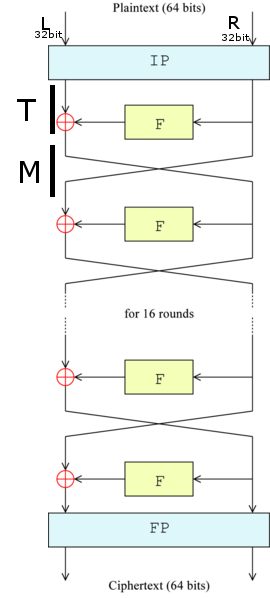
\includegraphics[width=5.5cm]{./bilder/DES-main-network.png}\\
  Schemata of the \em DES main network \em\\
  \vspace{2mm}
  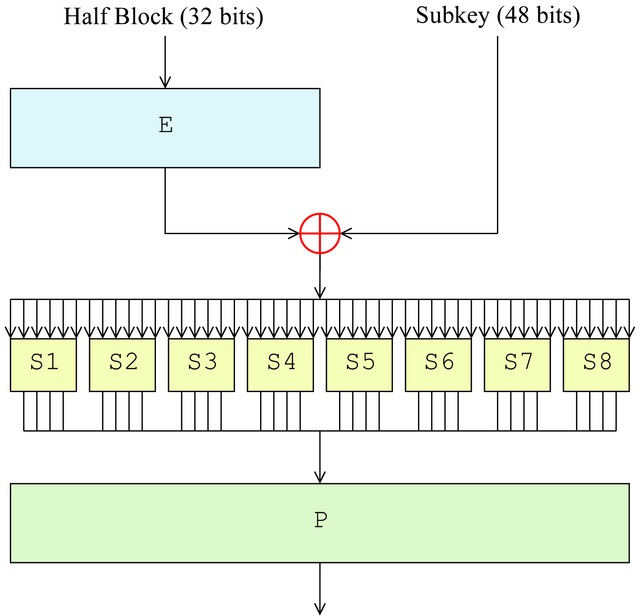
\includegraphics[width=7cm]{./bilder/DES-f-function.png}\\
  Schemata of the DES \em F-Box\em\\
 \end{center}
\end{minipage}

\subsection{PGP Pritty Good Privacy}
PGP is used for file encryption on a computer, computation of private and public RSA keys, and for sending and receiving of encrypted emails.\\
PGP is a set of different methods.\\
Necessary steps:
\begin{aufzaehlung}
\item A session key is generated.
\item The message is encrypted with a block cipher unsing the session key (IDEA and other block ciphers).
\item RSA is used to encrypt the session key with the public key of the receiver.
\item The encrypted message and the encrypted session key are bundled to a message that is mailed to the receiver.\\
\end{aufzaehlung}
PGP works without public key infrastructure (web of trust is used).

\subsubsection{Conclusion}
\begin{liste}
\item AES fast, RSA (based on Diffie-Hellmann) slow
\item AES need previous knowledge 
\item RSA for key-exchange, and AES/IDEA/DES for message cipher.
\end{liste}

\subsection{Hash Functions}
\begin{tabular}{l p{13cm}}
	collision				&	$h(x)=h(x')$. $kollision \approx \sqrt{2^n}=2^{n/2}$ Aufwand f\"ur Kollison ist ca. $2^{n/2}$ Rechenkomplexit\"at +
								$2^{n/2}$ Speicher. \\
							&	$h(x)$ ist Kollisionsresist, falls Aufwand eine Kollision zu finden ca. $2^{n/2}$ ist.\\
	preimage ressistant		&	Gegeben $Y$,(Fingerpint, Hashwert) Aufwand einen Input $X$ zu finden, 
								mit $Y=h(X)$ soll $\approx2^n$, $n$=Stringlaenge.\\

\end{tabular}

\section{MAC Message Authentication Codes}
Use parametrized hash function $\to$ $h_k: \sum^* \to \sum^4, x \to g(x) \oplus k$. $k$ is in this example a 4bit secret key.\\
Example: A would like to send a message to b, which isn't confidential, but sure, that the message wasn't changed during transmission.\\
\begin{tabular}{l}
	- $A$ and $B$ exchange a secret key k (strictly spoken, this exchange should be authenticated as well).\\
	- $A$ sends the message $m$ together with the MAC value $y=h_k(m)$ to $B$.\\
	- $B$ computes $y'=h_k(m')$ with the received message $m'$. $B$ accepts the message, if $y'=y$.
\end{tabular}
